% This is "sig-alternate.tex" V1.8 June 2007 Modified for SOUPS 2014
% This file should be compiled with V2.3 of "sig-alternate.cls" June 2007
%
% This example file demonstrates the use of the 'sig-alternate.cls'
% V2.3 LaTeX2e document class file. It is for those submitting
% articles to ACM Conference Proceedings WHO DO NOT WISH TO
% STRICTLY ADHERE TO THE SIGS (PUBS-BOARD-ENDORSED) STYLE.
% The 'sig-alternate.cls' file will produce a similar-looking,
% albeit, 'tighter' paper resulting in, invariably, fewer pages.
%
% ----------------------------------------------------------------------------------------------------------------
% This .tex file (and associated .cls V2.3) produces:
%       1) The Permission Statement
%       2) The Conference (location) Info information
%       3) The Copyright Line with ACM data
%       4) NO page numbers
%
% as against the acm_proc_article-sp.cls file which
% DOES NOT produce 1) thru' 3) above.
%
% Using 'sig-alternate.cls' you have control, however, from within
% the source .tex file, over both the CopyrightYear
% (defaulted to 200X) and the ACM Copyright Data
% (defaulted to X-XXXXX-XX-X/XX/XX).
% e.g.
% \CopyrightYear{2007} will cause 2007 to appear in the copyright line.
% \crdata{0-12345-67-8/90/12} will cause 0-12345-67-8/90/12 to appear in the copyright line.
%
% ---------------------------------------------------------------------------------------------------------------
% This .tex source is an example which *does* use
% the .bib file (from which the .bbl file % is produced).
% REMEMBER HOWEVER: After having produced the .bbl file,
% and prior to final submission, you *NEED* to 'insert'
% your .bbl file into your source .tex file so as to provide
% ONE 'self-contained' source file.
%
% ================= IF YOU HAVE QUESTIONS =======================
% Questions regarding the SIGS styles, SIGS policies and
% procedures, Conferences etc. should be sent to
% Adrienne Griscti (griscti@acm.org)
%
% Technical questions _only_ to
% Gerald Murray (murray@acm.org)
% ===============================================================
%
% For tracking purposes - this is V1.8 - June 2007

% --- Start page size ---
%Please use the following format  
\documentclass[twoside,letterpaper]{soups} 
\pdfpagewidth=8.5truein 
\pdfpageheight=11truein 
% --- End page size ---

\usepackage{graphicx}
\renewcommand{\topfraction}{0.99} % be more aggressive about text around floats
\renewcommand{\floatpagefraction}{0.99}
\pagestyle{plain} % page numbers

\usepackage{hyperref}

\usepackage{listings}

% proof conflicts with some other package
\let\proof\relax
\let\endproof\relax
\usepackage{amsthm}
\theoremstyle{definition}
\newtheorem{example}{Example}

\usepackage{booktabs}
\usepackage{todonotes}

\definecolor{grey}{rgb}{0.9,0.9,0.9}

\begin{document}
%
% --- Author Metadata here ---
\conferenceinfo{Symposium on Usable Privacy and Security
  (SOUPS)}{2014, July 9--11, 2014, Menlo Park, CA.}
\CopyrightYear{2014} % Allows default copyright year (200X) to be over-ridden - IF NEED BE.
%\crdata{0-12345-67-8/90/01}  % Allows default copyright data (0-89791-88-6/97/05) to be over-ridden - IF NEED BE.
% --- End of Author Metadata ---

\title{Analyzing Privacy of Android Apps}%
% \titlenote{(Produces the permission block, and copyright information). For use with SIG-ALTERNATE.CLS. Supported by ACM.}}
% \subtitle{Subtitle (optional)%
% \titlenote{A full version of this paper is available as
% \textit{Author's Guide to Preparing ACM SIG Proceedings Using
% \LaTeX$2_\epsilon$\ and BibTeX} at
% \texttt{www.acm.org/eaddress.htm}}}
%
% You need the command \numberofauthors to handle the 'placement
% and alignment' of the authors beneath the title.
%
% For aesthetic reasons, we recommend 'three authors at a time'
% i.e. three 'name/affiliation blocks' be placed beneath the title.
%
% NOTE: You are NOT restricted in how many 'rows' of
% "name/affiliations" may appear. We just ask that you restrict
% the number of 'columns' to three.
%
% Because of the available 'opening page real-estate'
% we ask you to refrain from putting more than six authors
% (two rows with three columns) beneath the article title.
% More than six makes the first-page appear very cluttered indeed.
%
% Use the \alignauthor commands to handle the names
% and affiliations for an 'aesthetic maximum' of six authors.
% Add names, affiliations, addresses for
% the seventh etc. author(s) as the argument for the
% \additionalauthors command.
% These 'additional authors' will be output/set for you
% without further effort on your part as the last section in
% the body of your article BEFORE References or any Appendices.

\numberofauthors{2} %  in this sample file, there are a *total*
% of EIGHT authors. SIX appear on the 'first-page' (for formatting
% reasons) and the remaining two appear in the \additionalauthors section.
%
\author{
% You can go ahead and credit any number of authors here,
% e.g. one 'row of three' or two rows (consisting of one row of three
% and a second row of one, two or three).
%
% The command \alignauthor (no curly braces needed) should
% precede each author name, affiliation/snail-mail address and
% e-mail address. Additionally, tag each line of
% affiliation/address with \affaddr, and tag the
% e-mail address with \email.
%
% 1st. author
\alignauthor
Gabriele Petronella\\
       \affaddr{University of Illinois at Chicago}\\
       % \affaddr{1932 Wallamaloo Lane}\\
       \affaddr{Chicago, Illinois}\\
       \email{gpetro3@uic.edu}
% 2nd. author
\alignauthor
Lenore D. Zuck\\
       \affaddr{University of Illinois at Chicago}\\
       % \affaddr{1932 Wallamaloo Lane}\\
       \affaddr{Chicago, Illinois}\\
       \email{zuck@uic.edu}
}
% There's nothing stopping you putting the seventh, eighth, etc.
% author on the opening page (as the 'third row') but we ask,
% for aesthetic reasons that you place these 'additional authors'
% in the \additional authors block, viz.
\additionalauthors{Additional authors: John Smith (The Th{\o}rv{\"a}ld Group,
email: {\texttt{jsmith@affiliation.org}}) and Julius P.~Kumquat
(The Kumquat Consortium, email: {\texttt{jpkumquat@consortium.net}}).}
\date{30 July 1999}
% Just remember to make sure that the TOTAL number of authors
% is the number that will appear on the first page PLUS the
% number that will appear in the \additionalauthors section.

\maketitle
\begin{abstract}
In this paper we present the design and the implementation of a tool to analyze privacy policies of Android applications, with the purpose of increasing the user's awareness about privacy-related concerns. The goal of this work is to produces a tool, targeted to users who wish to evaluate the compliance of arbitrary Android applications to their own privacy poli- cies. The tool implements a semantic analyzer of privacy policies, able to extract relevant sentences from them and put them in relationship with the corresponding privacy-related permissions requested by applications. This work was inspired by the manual review of privacy policies of Android applications, and noticing how a common informal structure was evident across multiple documents.
\end{abstract}


\section{Introduction}
\label{sec:intro}
During the last few years, mobile applications constantly growing in both number and importance in our everyday life.
Such impressive growth is marking a technology revolution, and, as many revolutions, it carries huge consequences affecting everyone's life. Some of this consequences lead to clear improvements, whereas some others put under spotlight some concerns that were not that relevant just a few years ago.
The increase in penetration and capabilities of mobile devices' has turned them in something most people would find hard to separate from, a sort of extension of their own body. Mobile devices nowadays typically hold a huge amount of information about their owner: email, contacts, bank accounts, social network profiles, location information.
How and under which circumstances such information can be disclosed has become a great concern very quickly, turning privacy related issues in notable examples of the aforementioned worrying consequences.

\subsection{Privacy awareness context}
We now define the scope in which this paper collocates itself, going through the main factor affecting privacy in mobile applications and describing the existing relationships between them.

We identify three main factors to take into consideration:
\begin{itemize}
       \item permissions
       \item actions and behaviors
       \item privacy policies
\end{itemize}

\emph{Permissions} determine which data or services the app can access on the user's device, so they effectively define the maximum potential impact an application can have over the user's privacy: the fewer the permissions, the lower the risk. However, a recent study \cite{stickley} showed how, given only the \texttt{INTERNET} permission, an Android application was capable of stealing online account login credentials.
This highlights how permissions only represent an upper bound: even apps requesting one single permission can significantly affect the privacy of user.

% As discussed in \autoref{sec:android-permission-model}, permissions are declared upfront by Android applications and they are visible prior to the app's installation.

We define \emph{actions} as the minimum unit of work an application can do. Actions can be divided in two main categories

\begin{itemize}
       \item actions that cannot be performed without an explicit permission
       \item actions that do not require an explicit permission to be performed  (e.g., impact local state of app)
\end{itemize}
The former category typically include the actions having any impact on the device's security. Such actions are forbidden by the OS (\emph{Operating System}) by default, and are allowed only if specific permissions have been granted to the application. The latter usually represent actions not affecting the device's security, e.g. actions confined within the bound of the internal application's logic.

We then define \emph{behaviors} as sequences of one or more actions; such definition implies that some behaviors, namely those including actions from the first category, can occur only when specific permissions have been granted.


\begin{example}
\leavevmode
Let us a consider a game application that stores user's top scores and sends them over the Internet to a remote server.
We can break this app down into the following actions:
\begin{itemize}
       \item \texttt{save\_user's\_top\_scores} ($A_1$)
       \item \texttt{send\_top\_scores\_over\_the\_internet} ($A_2$)
\end{itemize} 
The sequence of $A_1$ and $A_2$ forms the behavior \texttt{store\_and\_send\_user's\_top\_score\_to\_a\_remote\_sever} ($B_1$).
$A_1$ requires the permission \texttt{INTERNET} to be granted, whereas $A_2$ can always be performed.
This implies that $B_1$ can occur only if permission \texttt{INTERNET} is granted.
\end{example}

So we have seen how permissions enable actions and how actions can be composed to form behaviors. It is important to notice the cardinality of this relationships:
\begin{itemize}
       \item one permission enables one or more actions
       \item one behavior is enabled by one or more actions
\end{itemize}

Hence, it becomes evident how a many-to-many relationship between permissions and behaviors exist, i.e. enabling one or more permissions can potentially enable one or more behaviors.

While some of this behaviors are expected, and even desirable, some others might result unexpected and potentially undesirable. 

\begin{figure*}[ht]
\centering
     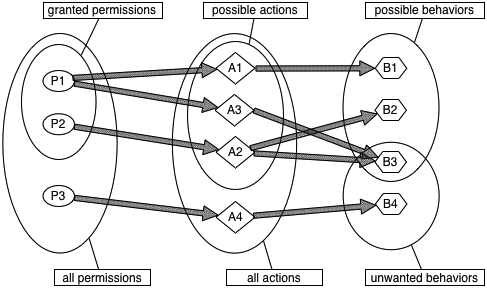
\includegraphics[width=0.9\textwidth]{images/context.png}
      \caption{Relationships between permissions, actions and behaviors}
      \label{fig:privacy-context}
\end{figure*}

\autoref{fig:privacy-context} highlights this possible scenario: permission $P_1$ is required to enable action $A_1$ which in turn enables behavior $B1$. Similarly, permission $P_2$ enables action $A_2$ and consequently behavior $B_2$. Granting permissions $P_1$, however, also enables action $A_3$, and when combined with action $A_2$, an unwanted behavior $B_3$ may occur.

Here is a practical instance of this scenario:
\begin{example}
\leavevmode
\label{ex:unwanted-behavior}
\begin{itemize}
       \item the \texttt{READ\_PHONE\_STATE} permission enables the action \texttt{detect\_an\_incoming\_phone\_call} ($A_1$), which enables the behavior \texttt{pause\_the\_game\_when\_an\_incoming\_phone\_call\_arrives} ($B_1$).
       \item the \texttt{INTERNET} permission enables the action \texttt{send\_and\_receive\_data\_over\_the\_Internet} ($A_2$), which enables the behavior \texttt{send\_the\_user's\_top\_score\_to\_a\_remote\_server} ($B_2$).
       \item the \texttt{READ\_PHONE\_STATE} permission also enables the action \texttt{read\_the\_user's\_phone\_number} ($A_3$). The combination of actions $A_2$ and $A_3$ enables the behavior \\ \texttt{send\_the\_user's\_phone\_number\_to\_a\_remote\_server}($B_3$), which may be undesirable.
\end{itemize} 
\end{example}

Given this potential issues with the permission-based model, it appears that something more has to be done in order to rule out unwanted behaviors.

This something that is commonly covered by privacy policies: legal documents provided together with the application. In the context we just described, privacy policies act should act as a filter on the possible behaviors, telling the final users which of the possible behaviors is the app going to actually generate.

For instance, a privacy policy may explicitly state that the user's phone number is never collected nor accessed, de facto promising the application will never perform \emph{A3}, hence ruling out \emph{B3}. Nonetheless, a real app may still deviate from what stated in its policy.

\section{Research scope and goals}
This paper restricts to Android applications, where permissions are declared upfront, as further explained in \autoref{sec:android-permission-model} when the application is installed.

This paper describes a methodology, supported by tools, that enables a user who installs an Android app to gain better understanding of the app's capabilities based on the permission it requires and its privacy policy, and alerts the user to some of the (potentially) unintended consequences that the user grants the application by installing it.

\subsection{Steps towards privacy awareness}
Given the general context of privacy awareness, we now identify a set of steps that are likely to lead to an increase in users' awareness.

\begin{enumerate}
       \item Understanding permissions \hfill \\
              Previous studies \cite{Felt:2012:APU:2335356.2335360} show how permissions are rarely understood by users. Specifically users appear not be able to correlate a permission with the possible actions it enables, let alone the spectrum of possible behaviors derived from actions interleaving.

              The first step towards awareness is to analyze permissions and derive potential consequences. We are especially interested in permissions that directly affect privacy. As an example, the \texttt{READ\_PHONE\_STATE} permission is typically requested by apps in order to be able to respond to phone events such as a incoming call, but it also enables the app to read the user's phone and IMEI numbers.

              Once permissions have been fully analyzed, one can then identify their  effect on the user's privacy.

       \item Correlating permissions and privacy policies \hfill \\
              The next step towards privacy awareness is to map each permission the app requests into its impact as stated in its privacy policy.
              While privacy policies do not share a common defined structure, they do express similar concepts in similar ways, which enable to extracting useful pieces of information from them. For example, an application requesting the \texttt{ACCESS\_FINE\_LOCATION} permission is very likely to be associated to a privacy policy containing expressions alike to \emph{``GPS'', ``Location Services'', `Global Positioning System', etc}.

              This step takes into consideration every permission that enables an app to affect the user's privacy with the final goal of building a dictionary of common expressions and patterns that associate the permission to natural language sentences in the privacy policy.

       \item Correlating apps behavior and privacy policies \hfill \\
              The last step is to monitor the app's actual behavior. Recalling Example \ref{ex:unwanted-behavior}, the application might never retrieve the user's phone number even though it requested such permission.

              This final step would then inform the users about the ``goodness'' of an application with respect the claims expressed in the privacy policy and the actual actions taken by the app once installed and running on their phone.
\end{enumerate}

\begin{figure*}[ht]
\centering
     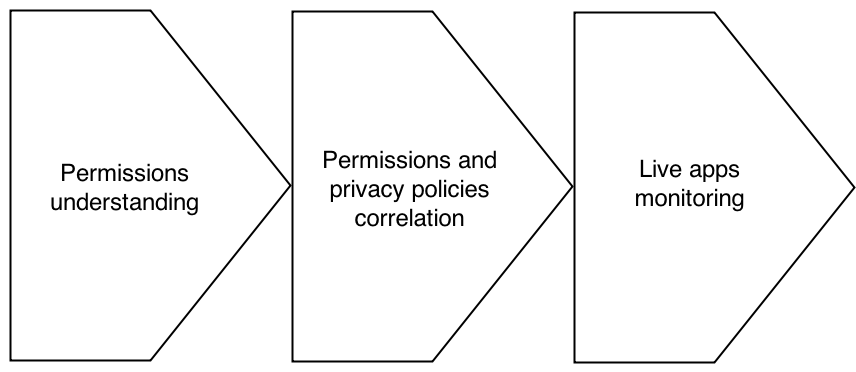
\includegraphics[width=0.8\textwidth]{images/awareness-steps.png}
      \caption{Privacy awareness steps}
      \label{fig:awareness-steps}
\end{figure*}

\subsection{Scope of this paper}
This paper focuses on the first two steps discussed in the previous section.

The first step requires an in-depth analysis and comprehension of the most requested permissions, in order to identify the potential privacy concerns each one of them carries.

Once the permissions of interest have been identified we will then perform a manual analysis in order to understand how privacy policies deal with the privacy concerns represented by them. The manual analysis will enable an automated process, which, given an arbitrary Android application published on the Play Store platform, retrieves its privacy policy and produces a human-readable report about the relationships between the permissions list and the analyzed legal document.

The final result will then allow a potential user to aggregate a large amount of privacy-related information in a quick and concise way, marking a clear step towards privacy awareness.

\subsection{Android OS Permission Model}
\label{sec:android-permission-model}
As explained in the Android Developer Guide \cite{android-developer-guide}, Android is a privilege-separated operating system, in which each application runs with a distinct system identity.

Additional finer-grained security features are provided through a ``permission'' mechanism that enforces restrictions on the specific operations that a particular process can perform, and per-URI permissions for granting ad-hoc access to specific pieces of data.

A basic Android application has no permissions associated with it by default, meaning it can not do anything that would adversely impact the user experience or any data on the device. To make use of protected features of the device the developer has to declare a list of permissions the application needs. Such list is specified in the \texttt{AndroidManifest.xml}, a file containing application metadata, included by every Android application.

For example, an application that needs to send and receive data over the Internet would specify:

\begin{lstlisting}[
float=*,
caption=Example of permission declaration in AndroidManifext.xml,
language=XML,
backgroundcolor=\color{grey}
]
<manifest xmlns:android="http://schemas.android.com/apk/res/android"
    package="com.android.app.myapp" >
    <uses-permission android:name="android.permission.INTERNET" />
    ...
</manifest>
\end{lstlisting}

At application install time, permissions requested by the application are granted to it by the package installer, based on checks against the signatures of the applications declaring those permissions and/or interaction with the user.
No checks with the user are done while an application is running: it either was granted a particular permission when installed, and can use that feature as desired, or the permission was not granted and any attempt to use the feature will fail without prompting the user.

\section{Related Work}
As discussed in \autoref{sec:android-permission-model}, permissions are granted at install time, meaning that a user is supposed to have reviewed the permissions the application requested and to have deemed them acceptable, before granting them altogether.

Such mechanism has been criticized for several reasons: first of all, recent studies \cite{Felt:2012:APU:2335356.2335360} \cite{Kelley:2012:CPI:2426020.2426027} show how users might not have complete understanding of the meaning and consequences of each permission in the list. The same studies also show how even experienced users are found not pay attention to the permission list, most likely due to its verbosity and length. To further prove this last observation, in recent experiment \cite{stickley} an ad-hoc application was developed and put on the Play Store; the application requested all possible permissions, enabling the researchers to steal personal data from the user, such as email address and phone numbers. The application received 1300 downloads over a 3-month period, without being advertised, and collected 1950 email addresses.

\section{Approach}
\label{sec:overview}
In this section we will discuss the analysis approach in details. Two well-distinct stages of such analysis can be identified, namely a manual one and an automated one.
The manual analysis involves an accurate investigation of Android permissions and their relationship with privacy policies.

The outcome of this first stage is a formal representation of this relationship, which enables the second - automated - phase of the analysis, thoroughly discussed in \autoref{sec:automated-analysis}.

%%%%%%%%%%%%%%%%%%%%%%%%%%%%%%%%%%%%%%%%%%
\subsection{Manual analysis}
In this section we present the manual steps that needed to be executed in order to enable an automated analysis.

\subsubsection{Permissions of Interest}
The first step in our research is to identify which of the permissions an app can request have privacy related consequences.

Firstly we are interested into discovering which are the most requested permissions in our domain of interest.
There are no official data released by Google, however we were able to retrieve empirical data with the use of
unofficial APIs \cite{play-store-unofficial-api}, discussed in greater details in \autoref{sec:implem}.

The Play Store platform divides apps in categories (such as \emph{Games}, \emph{Education}, \emph{Tools} and so on). We run
an analysis on the top downloaded free apps for each categories, identifying a total of 4300 applications;
we then retrieved the permission list for each one of them and aggregated such data. The top 20 requested permissions are shown in \autoref{tab:top20-permissions}.

\begin{table}[ht]
    \caption{TOP 20 REQUESTED PERMISSIONS IN FREE APPS}
    \label{tab:top20-permissions}
    \centering
    \begin{tabular}{clc}
        \toprule
            \#   & Permission & \% apps using it \\
            \midrule
                1  & INTERNET                       &   99.35\% \\
                2  & ACCESS\_NETWORK\_STATE         &   98.35\% \\
                3  & READ\_EXTERNAL\_STORAGE        &   92.35\% \\
                4  & WRITE\_EXTERNAL\_STORAGE       &   92.35\% \\
                5  & ACCESS\_WIFI\_STATE            &   85.47\% \\
                6  & READ\_PHONE\_STATE             &   78.39\% \\
                7  & WAKE\_LOCK                     &   59.65\% \\
                8  & VIBRATE                        &   32.79\% \\
                9  & GET\_ACCOUNTS                  &   32.79\% \\
                10 & ACCESS\_COARSE\_LOCATION       &   19.86\% \\
                11 & GET\_TASKS                     &   14.86\% \\
                12 & RECEIVE\_BOOT\_COMPLETED       &   13.88\% \\
                13 & ACCESS\_FINE\_LOCATION         &   9.93\%  \\
                14 & READ\_LOGS                     &   9.88\%  \\
                15 & MOUNT\_UNMOUNT\_FILESYSTEMS    &   6.93\%  \\
                16 & RECORD\_AUDIO                  &   5.95\%  \\
                17 & CHANGE\_WIFI\_STATE            &   4.98\%  \\
                18 & DISABLE\_KEYGUARD              &   4.95\%  \\
                19 & READ\_CONTACTS                 &   3.00\%  \\
                20 & WRITE\_SETTINGS                &   2.98\%  \\
        \midrule
            \multicolumn{3}{c}{\footnotesize \emph{Generated from 4300 apps on Nov 17, 2013}} \\
        \bottomrule
    \end{tabular}
\end{table}

The general list of permissions, however, includes permissions with no significant impact with respect to privacy matters. The next step in our research is then to identify which permissions affect the user's privacy and how.

What follows is a list of all the permissions which enable actions raising privacy concerns. For each permission a list of enabled actions is provided along with a discussion about the privacy concerns.

\begin{description}
    \item[INTERNET] \hfill
        \begin{description}
             \item[Actions enabled] \hfill
                \begin{itemize}
                     \item send data over the Internet
                     \item receive data over the Internet
                 \end{itemize} 
             \item[Privacy concerns]
                This permission is the most requested and also the most dangerous, privacy-wise, as it enables the communication with remote servers over the Internet.
                Used in combination with other permissions it allows the application to send any retrieved data to an arbitrary remote server.
             \item[Examples]
                An application can send any sensitive data retrieved thanks to other permissions over the Internet. For instance on can think of an application reading the user's phone number and sending it to a remote server, perhaps with the purpose of targeted phone advertisement.
                As described in a recent study \cite{stickley}, this permission can be dangerous by itself.
         \end{description} 
   
   \item[READ\_EXTERNAL\_STORAGE] \hfill
        \begin{description}
             \item[Actions enabled] \hfill
                \begin{itemize}
                     \item read files on the external SD card
                 \end{itemize} 
             \item[Privacy concerns]
                This permission allows to read files on an external SD card, so that anything stored in the external memory can be accessed by the app, including pictures, videos and data stored by other applications.
             \item[Examples]
                An application can retrieve all the user's picture stored on the SD card and send them to a remote server, violating the user's privacy.
         \end{description} 
    
    \item[WRITE\_EXTERNAL\_STORAGE] \hfill
        \begin{description}
             \item[Actions enabled] \hfill
                \begin{itemize}
                    \item write files on the external SD card
                    \item read files on the external SD card
                 \end{itemize} 
             \item[Privacy concerns]
                Despite the name, this permission implicitly enables also \texttt{READ\_EXTERNAL\_STORAGE}, so the same privacy concerns apply.
         \end{description} 

    \item[ACCESS\_WIFI\_STATE] \hfill
        \begin{description}
             \item[Actions enabled] \hfill
                \begin{itemize}
                    \item access the \texttt{WifiManager}
                 \end{itemize} 
             \item[Privacy concerns]
                Accessing the \texttt{WifiManager} allows the app to read information about the WiFi network the device is connected to, including the current IP address.
             \item[Examples]
                One can think of an application tracking the user's location by estimating the WiFi network's location, as recent studies demonstrate \cite{Yang:2008:ELU:1339822.1339967}
         \end{description} 

    \item[READ\_PHONE\_STATE] \hfill
        \begin{description}
             \item[Actions enabled] \hfill
                \begin{itemize}
                    \item detect in-progress phone calls
                    \item read IMEI and IMSI identifiers
                    \item read the network provider information
                    \item read the user's phone number
                 \end{itemize} 
             \item[Privacy concerns]
                This is one of the most controversial permissions. While most applications request this permission in order to detect incoming phone calls, which is usually a legitimate use, it can also be used to retrieve sensitive pieces of information such as the phone number.
             \item[Examples]
                An application can steal the user's phone number and sell it to advertisement companies for profit.

         \end{description} 

    \item[GET\_ACCOUNTS] \hfill
        \begin{description}
             \item[Actions enabled] \hfill
                \begin{itemize}
                    \item read the list of accounts from the Accounts Service
                 \end{itemize} 
             \item[Privacy concerns]
                The list of accounts consists of a list of usernames for each account associated with the device. For instance, the application might retrieve the email address associated with the user's GMail account.
             \item[Examples]
                Retrieving account's usernames can be the first step towards identity stealing. A malicious application can use this piece of information to break into a user's email account and access personal data.
         \end{description} 

    \item[ACCESS\_COARSE\_LOCATION] \hfill
        \begin{description}
             \item[Actions enabled] \hfill
                \begin{itemize}
                    \item know the (coarse) device location
                 \end{itemize} 
             \item[Privacy concerns]
                The coarse location is determined by the triangulation of GSM tower cells information and WiFi information. Although coarse the location can determine a user's location with a good level of accuracy, therefore representing a privacy concern.                
         \end{description}

    \item[GET\_TASKS] \hfill
        \begin{description}
             \item[Actions enabled] \hfill
                \begin{itemize}
                    \item know which tasks are running or recently run
                 \end{itemize} 
             \item[Privacy concerns]
                Allows an application to get information about the currently or recently running tasks. While not dangerous by itself, it can help in stealing information when combined with other permissions.
         \end{description} 

    \item[ACCESS\_FINE\_LOCATION] \hfill
        \begin{description}
             \item[Actions enabled] \hfill
                \begin{itemize}
                    \item know the (fine) device location
                 \end{itemize} 
             \item[Privacy concerns]
                The same privacy concerns as coarse location apply.
         \end{description} 

    \item[READ\_LOGS] \hfill
        \begin{description}
             \item[Actions enabled] \hfill
                \begin{itemize}
                    \item read the low-level system log files
                 \end{itemize} 
             \item[Privacy concerns]
                Not particularly worrying by itself, but it enables the app to read everything other applications might have logged. If some application logs sensible data, this permission will allow them to be read.
         \end{description} 

    \item[RECORD\_AUDIO] \hfill
        \begin{description}
             \item[Actions enabled] \hfill
                \begin{itemize}
                    \item record audio
                 \end{itemize} 
             \item[Privacy concerns]
                While this permission has legitimate uses such as note taking apps or voice search apps, it is a potential tool for eavesdropping and recording of sensible information. 
         \end{description}   

    \item[READ\_CONTACTS] \hfill
        \begin{description}
             \item[Actions enabled] \hfill
                \begin{itemize}
                    \item read the user's contacts data.
                 \end{itemize} 
             \item[Privacy concerns]
                The whole user's address book can be read. 
         \end{description}  

\end{description}

Table \autoref{tab:top-privacy-related-permissions} summarizes the privacy-related permissions we will consider in our analysis.

\begin{table}[ht]
    \caption{TOP PRIVACY-RELATED PERMISSIONS IN FREE APPS}
    \label{tab:top-privacy-related-permissions}
    \centering
    \begin{tabular}{clc}
        \toprule
            \#   & Permission & \% apps using it \\
            \midrule
                1  & INTERNET                       &   99.35\% \\
                2  & READ\_EXTERNAL\_STORAGE        &   92.35\% \\
                3  & WRITE\_EXTERNAL\_STORAGE       &   92.35\% \\
                4  & ACCESS\_WIFI\_STATE            &   85.47\% \\
                5  & READ\_PHONE\_STATE             &   78.39\% \\
                6  & GET\_ACCOUNTS                  &   32.79\% \\
                7  & ACCESS\_COARSE\_LOCATION       &   19.86\% \\
                8  & GET\_TASKS                     &   14.86\% \\
                9  & ACCESS\_FINE\_LOCATION         &   9.93\%  \\
                10 & READ\_LOGS                     &   9.88\%  \\
                11 & RECORD\_AUDIO                  &   5.95\%  \\
                12 & READ\_CONTACTS                 &   3.00\%  \\
        \midrule
            \multicolumn{3}{c}{\footnotesize \emph{Generated from 4300 apps on Nov 17, 2013}} \\
        \bottomrule
    \end{tabular}
\end{table}

\subsubsection{Relationship with privacy policy}
Now that we identified the permissions we are interested in, we want to see how each permission relates to the privacy policy, i.e. in which terms the privacy policy deals with permissions the app requested.

Our analysis involved an initial corpus of twenty policies. For each permission we went through each privacy policy of the corpus, manually extracting common pattern and terms.

The result of this manual investigation is a lookup table associating each permission with a list of common words or expressions used in the privacy policies to refer to the actions enabled by it.

\paragraph{Example: Rovio's Privacy Policy}
We now illustrate what expressed in the previous section, taking a popular app's privacy policy as an example. The application in question is \emph{Angry Birds} by Rovio Entertainment Ltd. If we take the \texttt{ACCESS\_COARSE\_LOCATION} permission into consideration we can find several parts of the privacy policy referring to it. Once such parts have been identified, the relevant words and expressions concerning the specific matter are then extracted. What follow are the relevant sections of Rovio's privacy policy concerning the user's location matter:

\begin{quote}
\emph{Rovio or third parties operating the ad serving technology may use demographic and \textbf{geo-location} information (for more information regarding use of Location Data see below Section 3) as well as information logged from your hardware or device to ensure that relevant advertising is presented within the Service.}
\end{quote}

\begin{quote}
\emph{To the extent Rovio makes \textbf{location} enabled Services available and you use such Services, Rovio may collect and process your \textbf{\textbf{location}} data to provide \textbf{location} related Services and advertisements.}
\end{quote}

\begin{quote}
\emph{The \textbf{location} data is processed and stored only for the duration that is required for the provision of the \textbf{location} related Services.}
\end{quote}

\begin{quote}
\emph{Rovio may use, depending on the service (1)IP-based \textbf{location} based on the IP address presented by the end-user, (2) fine \textbf{geo-location} data based on coordinates obtained from a mobile device's \textbf{GPS} radio, or (3) coarse, network-based \textbf{geo-location} data based on proximity of network towers or the \textbf{location} of WiFi networks.}
\end{quote}

\begin{quote}
\emph{Your fine, \textbf{GPS-based} \textbf{geo-location} is not accessed without your consent.}
\end{quote}

\begin{quote}
\emph{Notwithstanding Rovio's partners who are providing location related parts of the Service, Rovio will not share your GPS geo-location with third parties without your consent.}
\end{quote}

\begin{quote}
\emph{To the extent Rovio makes available GPS geo-location to third parties in accordance with this Privacy Policy, it will be provided anonymously.}
\end{quote}

\begin{quote}
\emph{This includes, for example, collection of IP-based geolocation data to ensure that the product, service or features served comply with applicable laws of that nation.}
\end{quote}

All of the above sentences are relevant to the matter of establishing what is the app expected behavior with respect to the user's location information. It is particularly interesting to observe a few characteristics of some of the cited sentences. Specifically Rovio's privacy policy states

\emph{Your fine, \textbf{GPS-based} \textbf{geo-location} is not accessed without your consent.}

This provides a false sense of assurance, since in Android application the consent has already been given at installation time, so the geo-location can always be accessed by the application without further notice to the user.

\paragraph{Example: Halfbrick's Privacy Policy}
Similar examples can be found in many popular apps. Let us for instance consider the case of Halfbrick, a company most known for a game called Fruit Ninja. It the app's privacy policy one can read

\emph{Where you allow us access to such information, we may also collect information from your device such as your geographic location}

Again, we can see how similar matters are mentioned similarly in different privacy policies, and also how again such sentence provides false assurance: Android apps always have permissions granted upfront, so the phrase \emph{``Whenever you allow us''}, realistically means \emph{``Whenever the app is installed''} on an Android device.

\subsubsection{Lookup table example}
Based on this manual analysis we built a look up table of permissions and the way they are referred to in policies. An sample entry of this table is shown in \autoref{tab:lookup-coarse-location}.

\begin{table}[ht]
    \caption{ACCESS\_COARSE\_LOCATION LOOKUP TABLE}
    \label{tab:lookup-coarse-location}
    \centering
    \begin{tabular}{lp{4cm}}
        \toprule
            Permission   & Keywords \\
            \midrule
                \texttt{ACCESS\_COARSE\_LOCATION}  & \emph{``gps''}, \emph{``IP based location''}, \emph{``location''}, \emph{``location services''}, \emph{``geo-location''}, \emph{``geographic location''} \\
        \bottomrule
    \end{tabular}
\end{table}

\subsection{Automated analysis}
\label{sec:automated-analysis}
Once the lookup table has been constructed is then possible to proceed with an automated analysis of applications.
In this section we present the high level steps taken by the analysis, along with the challenges face during this process, while the implementation details will be discussed in \autoref{sec:implem}.

\subsubsection{Privacy policy retrieval}
The first step is to retrieve the privacy policy given an arbitrary application. This proved to be one significant challenge, for the following main reasons:
\begin{itemize}
    \item there is no legal requirement enforcing an Android application to have a privacy policy. Some application simply don't provide one.
    \item there is no standard format for such documents. While the Play Store has a standard interface for providing a link to an app's privacy policy, the content of the link itself is arbitrary and completely at the discretion of the developer.
    \item some application developers do not provide a link to the privacy policy in the Play Store.
\end{itemize}

For the purposes of this research work, we limit our search for the privacy policy to the Play Store web interface. If the developer provided a privacy policy link, it is followed through and analyzed, otherwise the search fails and we assume the application not to have a privacy policy at all. This may not hold true and it is a known downside of this approach, which can be object of further improvement in future development of this analysis.

When present, the \emph{Privacy Policy} link in the Play Store interface can be followed to access the actual document, which can then be fetched in order to perform semantic analysis over it, as discussed in \autoref{sec:privacy-policy-analysis}.

\subsubsection{Permissions retrieval}
The next step of the analysis involves retrieving the permissions list given an arbitrary Android application. This is a much easier task than retrieving the privacy policy, since every Android application is guaranteed to declared the requested permissions in an uniform format. The main challenge of this step regards the implementation, due to the lack of official APIs to retrieve such piece of information. The details about how this issue was overcome are provided in \autoref{sec:implem}.

\subsubsection{Privacy policy analysis}
\label{sec:privacy-policy-analysis}
Once the privacy policy document and the permissions list are both available, we can then proceed with the semantic analysis.

Firstly, the document is broken down into semantic sections, such as paragraphs and sentences.
Secondly the keyword and expressions contained in the lookup table of each permission are matched against each section.
For each permission the relevant matching sentences are then collected.

Such result is then presented to the final user, as discussed in the next section.

\subsubsection{User's interface}
The automated analysis is made available to the user via a web interface. The interface allows the user to search for an arbitrary application on the Play Store; the permissions list and the privacy policy are then automatically retrieved, whenever possible.
The user has then the ability of selecting a specific permission, and a list of relevant sentences will be extracted by the privacy policy and presented to them, along with an accurate description of the permission itself.

Such interface allows the user to quickly evaluate the privacy-related risks of an Android application, by highlighting the relevant sections of the privacy policy and by providing useful information about sensible permissions.

%%%%%%%%%%%%%%%%%%%%%%%%%%%%%%%%%%%%%%%%%%
\subsection{Example}
We now present an example in order to better summarize the steps discussed in the previous section.
\autoref{fig:example-search} shows the search interface: in the example we are searching for the game \emph{Angry Birds} and, as we digit, a list of suggestions is dynamically computed by live-querying the Play Store and presented to the user.

\begin{figure}[ht]
\centering
     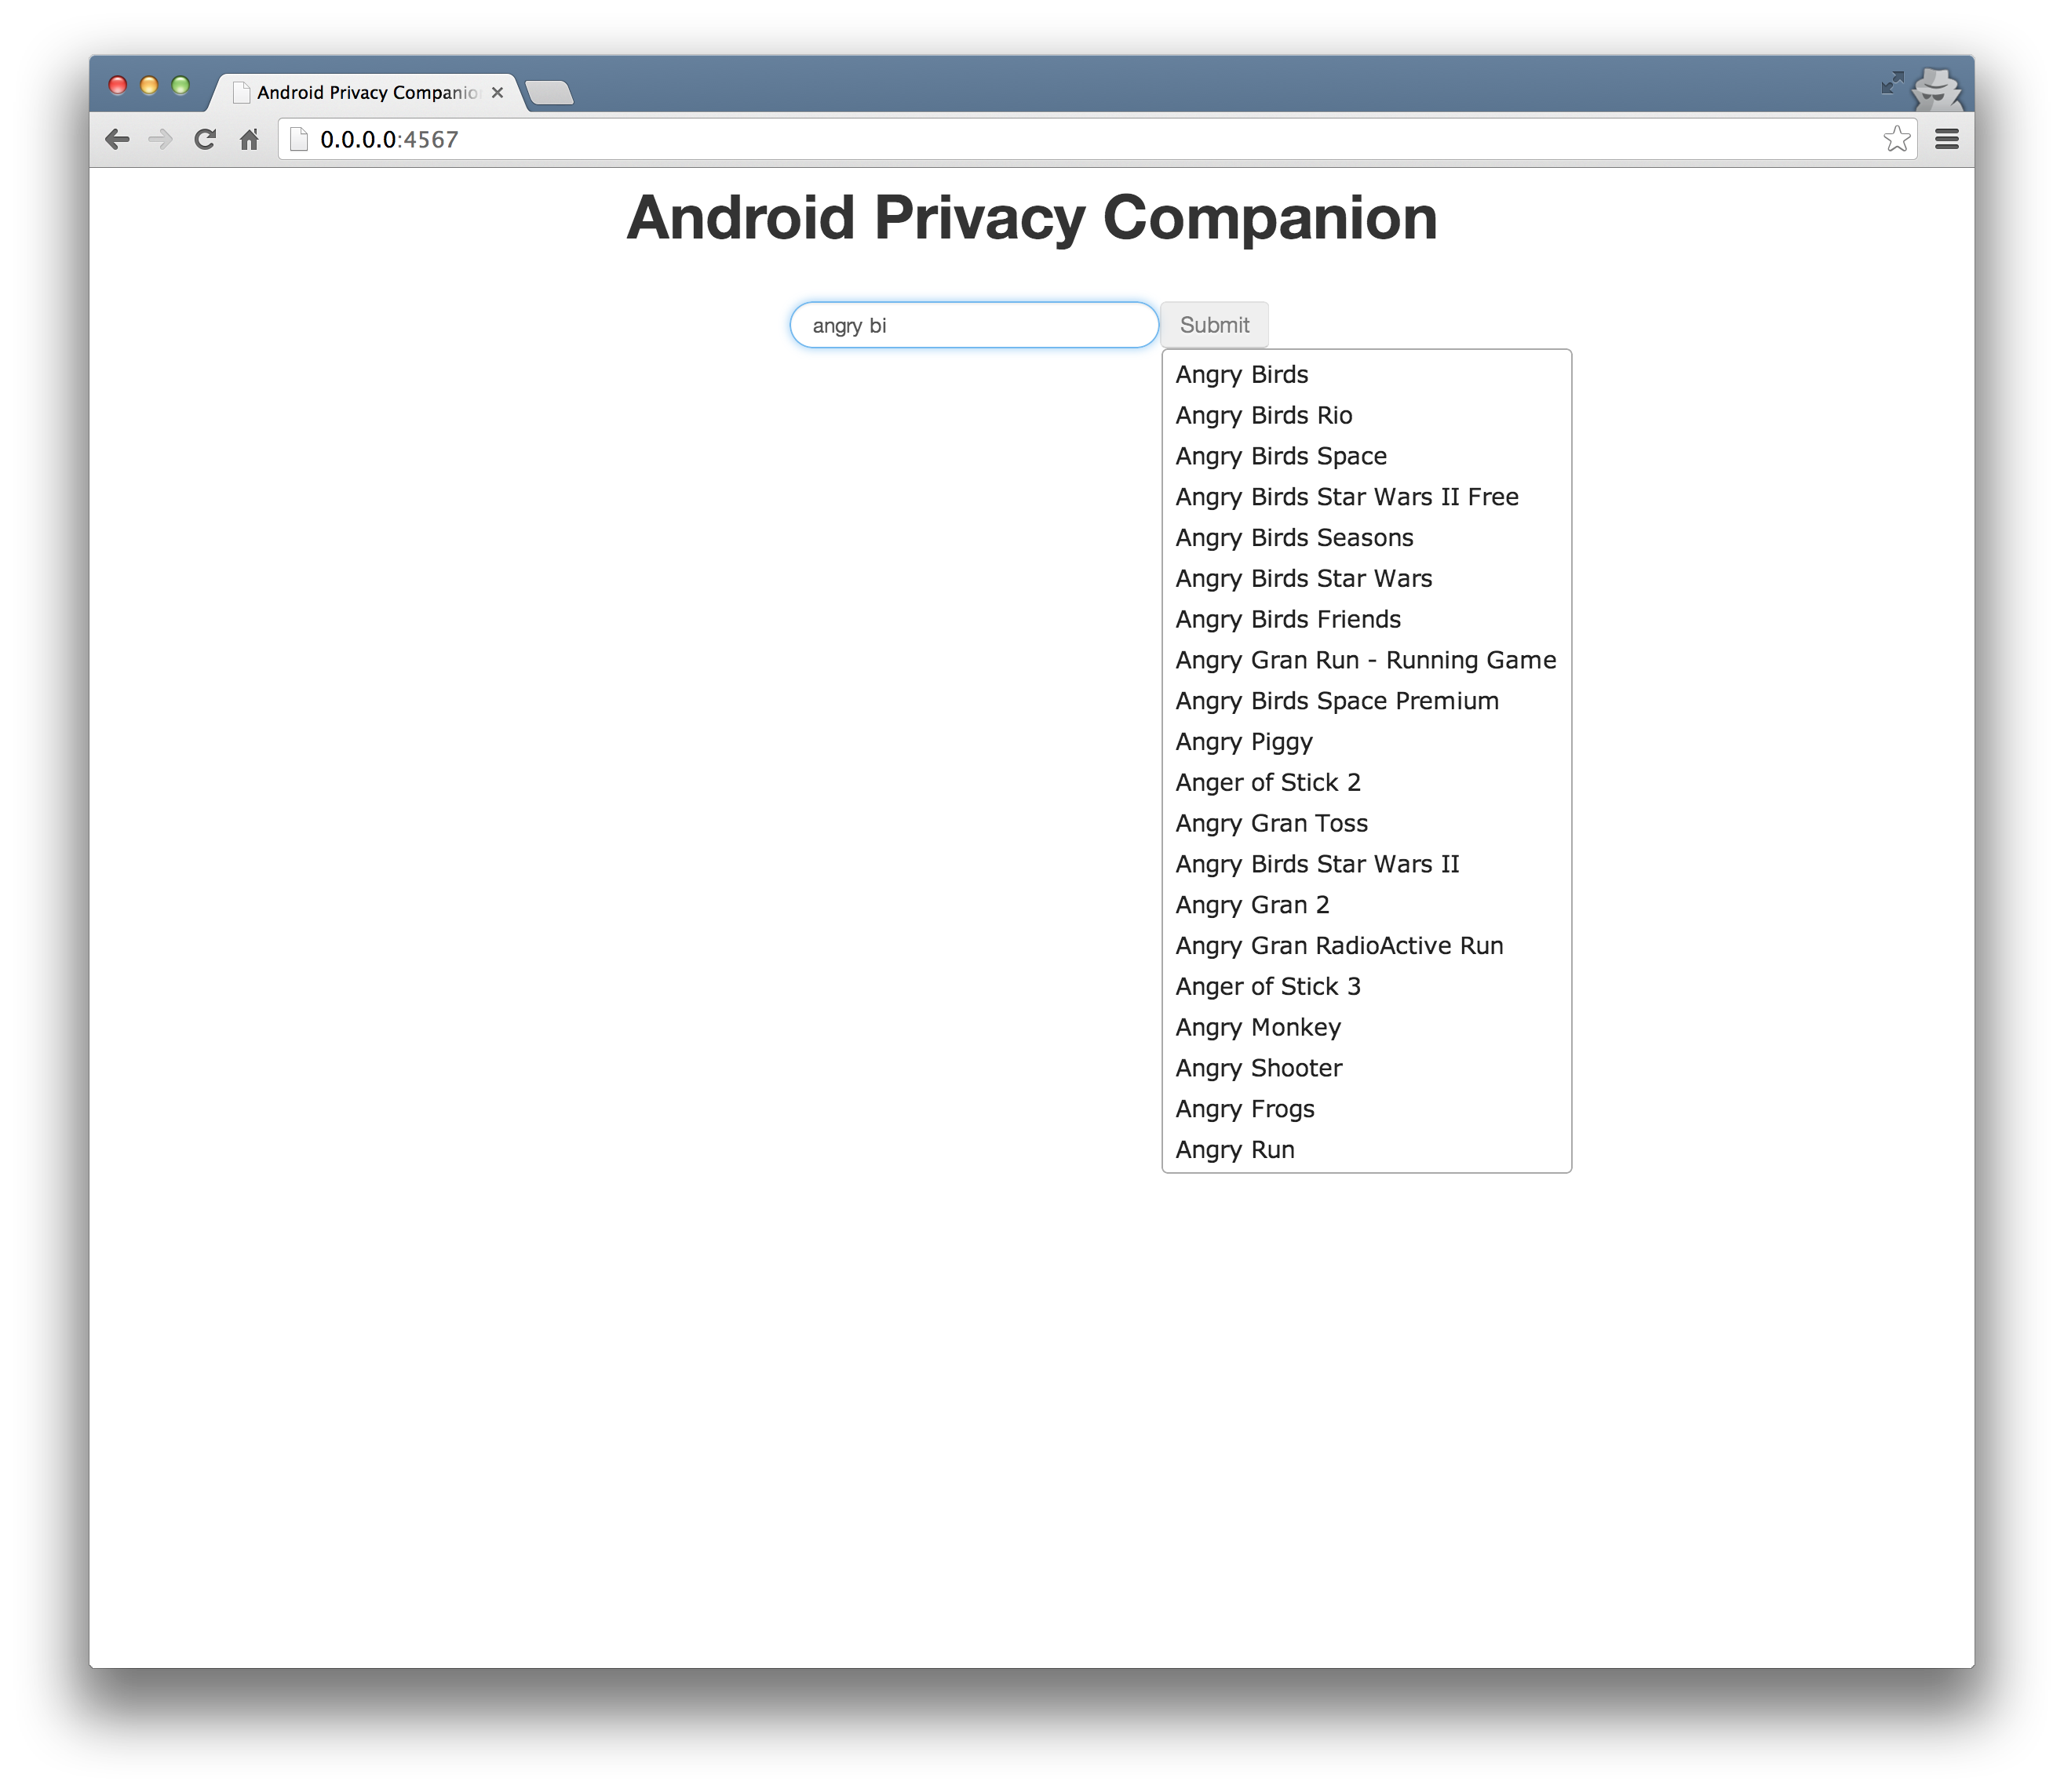
\includegraphics[width=\linewidth]{images/example-search}
      \caption{Search interface}
      \label{fig:example-search}
\end{figure}

Once the application has been selected from the list, the permissions list and the privacy policy are automatically retrieved and displayed.
The user can then select one of the permissions requested by the application in order to see all the relevant sections of the privacy policy.

In \autoref{fig:example-permission-selected} the user selected the \texttt{ACCESS\_COARSE\_LOCATION} permission and a list of relevant sentences is displayed right under the permission description.

\begin{figure}[ht]
\centering
     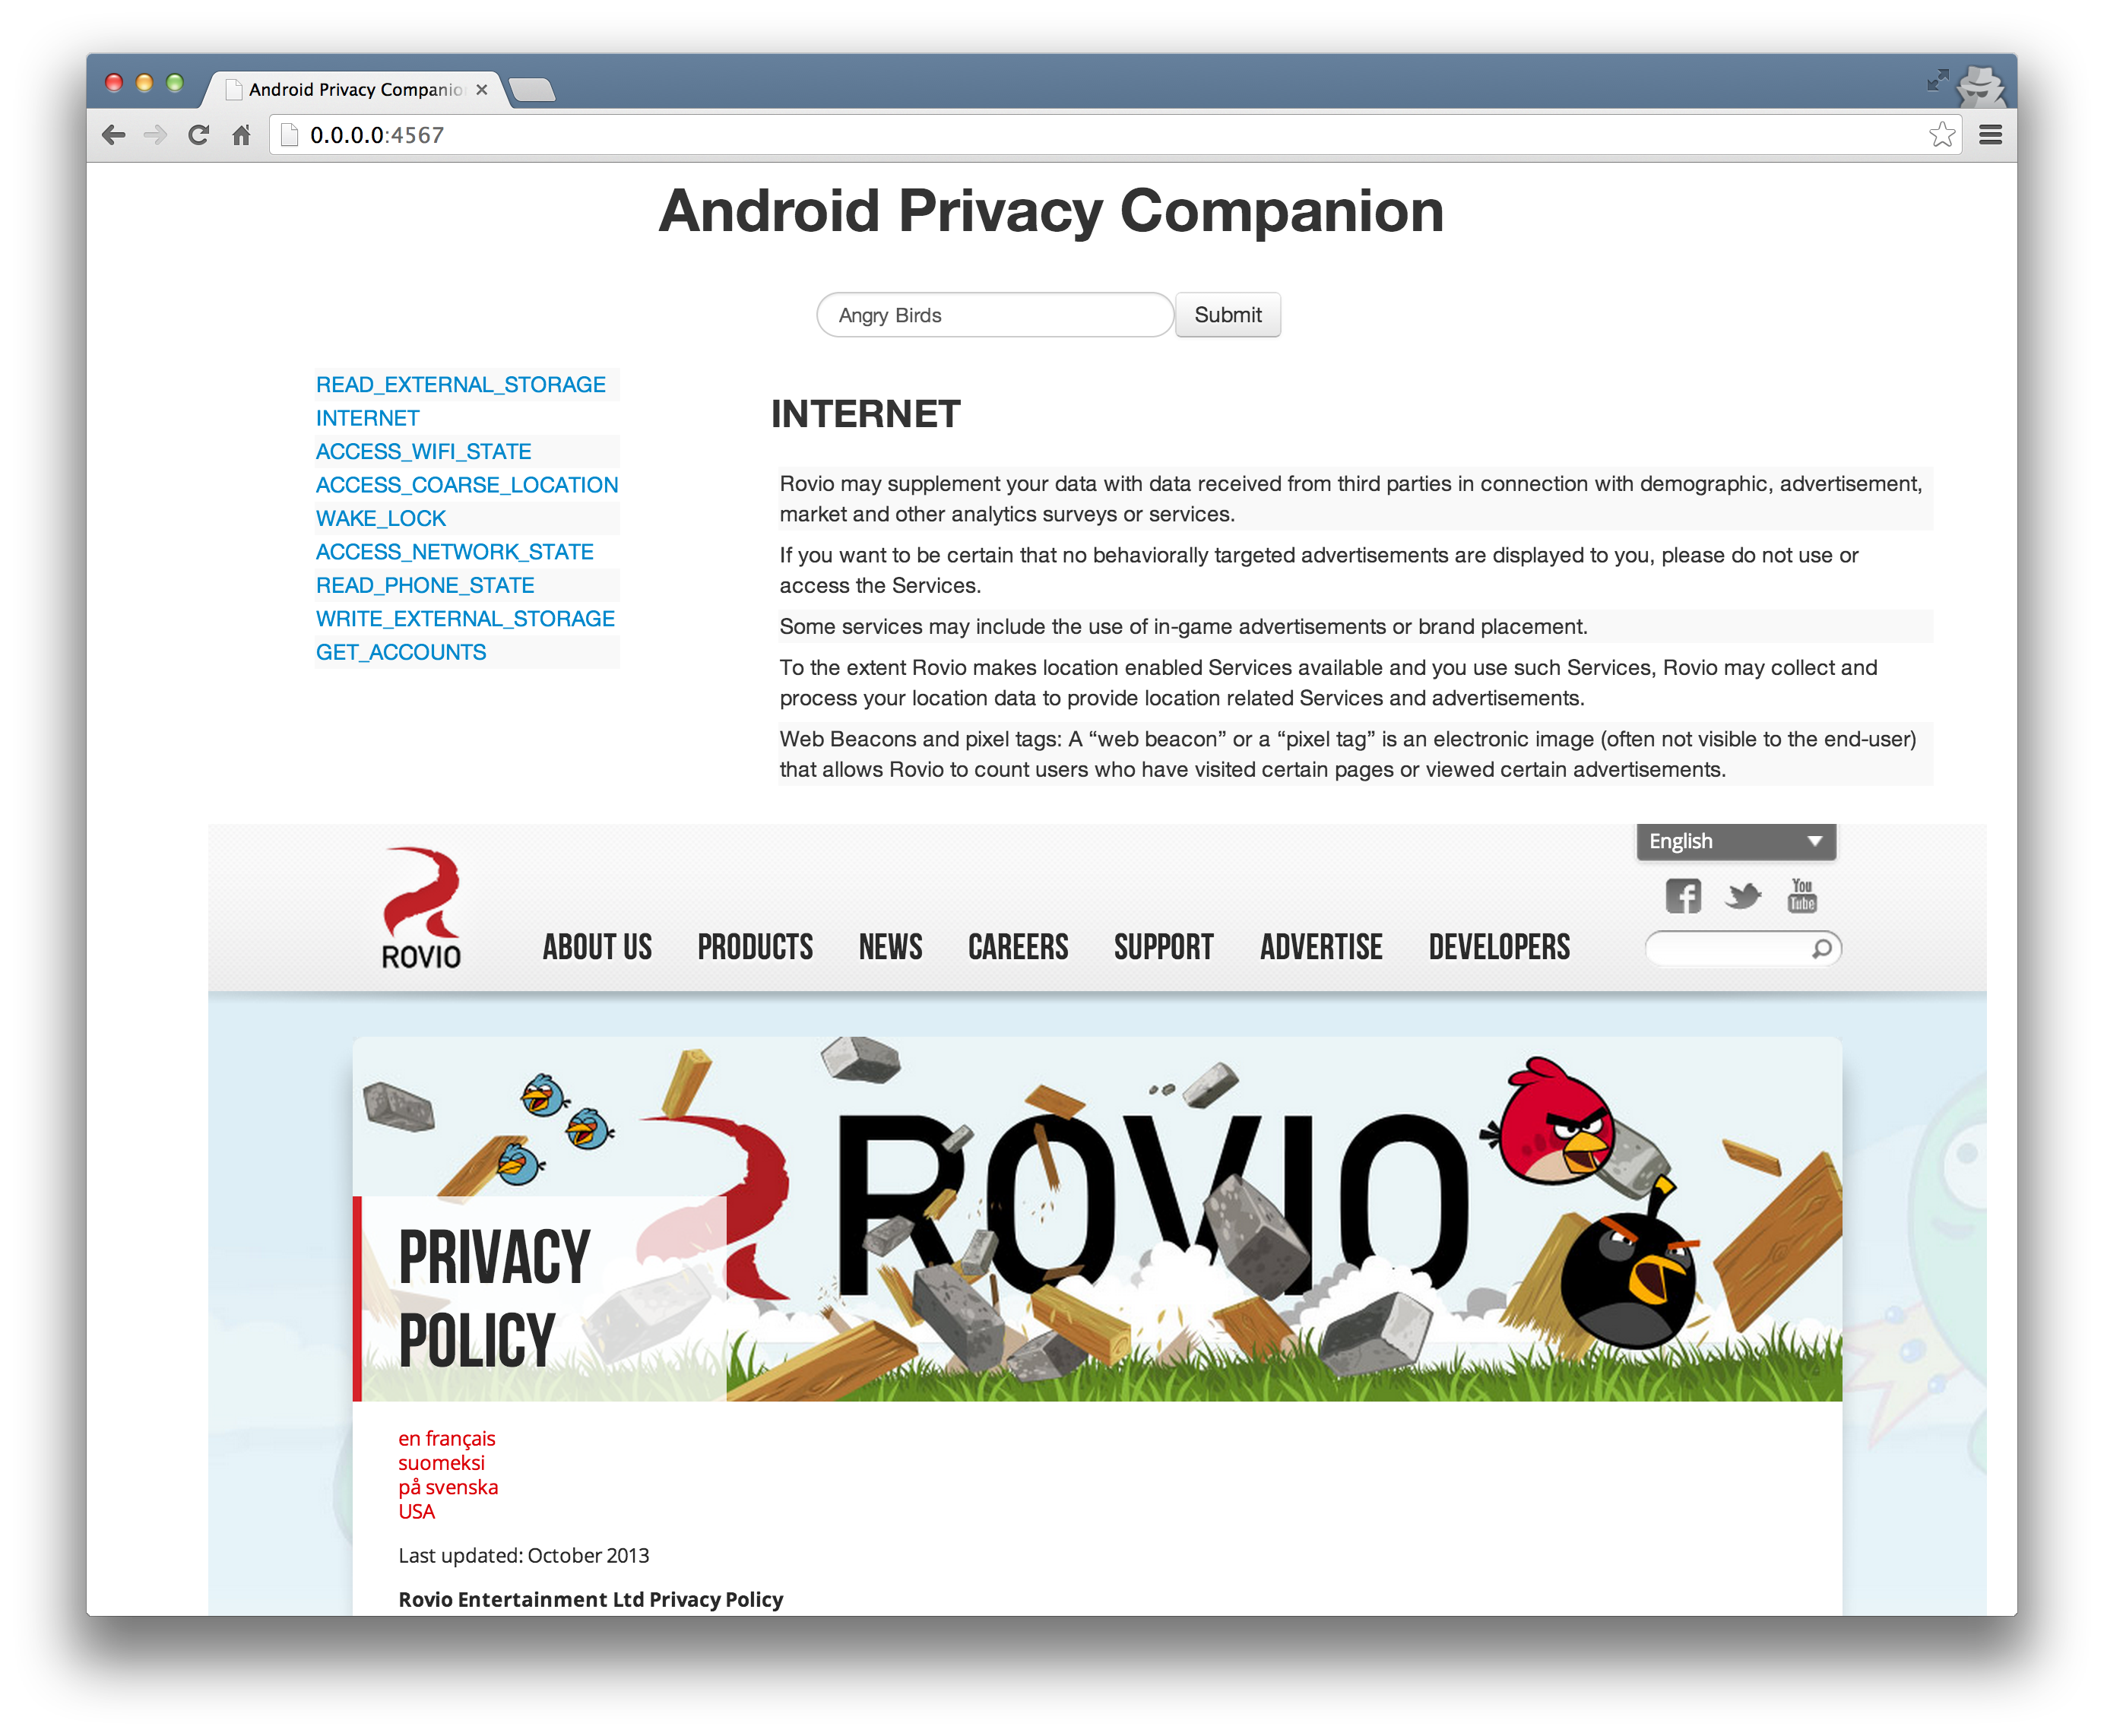
\includegraphics[width=\linewidth]{images/example-permission-selected}
      \caption{Permission display interface}
      \label{fig:example-permission-selected}
\end{figure}

\section{Implementation}
\label{sec:implem}
In this section we present the details of the implementation. We first describe the data collection process, for privacy policies and permissions; we then discuss how the data collected were subsequently analyzed, preprocessed and selected. Finally we present the implementation of the algorithm discussed in the previous sections.

\subsection{Permissions collection}
\label{sec:permissions-collection}
As discussed in \autoref{sec:android-permission-model}, Android apps are required to declare upfront a list of permissions they need. Such list is stored in the \texttt{AndroidManifest.xml} file of each app. At installation time the user is able to review the permissions and decide whether to grant them or not.

Due to the lack of public official API for retrieving the permissions list, we first attempted to retrieve it through the Play Store web interface.

From a programmatic point of view, however, some issues arise. First of all the permissions as presented to the user are in a natural language format, whereas the permissions in the \texttt{AndroidManifest.xml} file are expressed with a canonical name. For instance the permission \texttt{READ\_EXTERNAL\_STORAGE} correspond to the natural language description \emph{``modify or delete the contents of your USB storage''}.
This would require an extra processing step to map the natural language description to the correspondent.

Secondly, and most importantly, the permission list is accessible from the web interface only after pressing the install button and this step is allowed only from a registered Google account with at least one Android device registered.

While this issues can be overcome, they added unexpected complexity to this step and therefore an alternative path was explored.

As mentioned above, Google does not provide an official API for retrieving applications metadata, such as the permission list, however an unofficial Python implementation exist and it is publicly available \cite{play-store-unofficial-api}. There also exist another open-source project \cite{play-store-crawler}, based on the unofficial API, featuring the ability of performing search queries, downloading apps and retrieving apps permissions.

Thank to the use of the unofficial API, the issues mentioned above were solved and we were able to retrieve the permissions from an arbitrary app available on the Play Store.

%%%%%%%%%%%%%%%%%%%%%%%%%%%%%%%%%%%%%%%%%%
\subsection{Privacy Policy collection}
\label{sec:pp-collection}
Automatically retrieving a privacy policy document for an arbitrary Android app is a much harder task than retrieving its permission list.

Whenever present, the Privacy Policy link appears in the \emph{Additional Information} section on the Play Store web interface, as shown in \autoref{fig:play-store-privacy-link}.

\begin{figure*}[b!]
\centering
     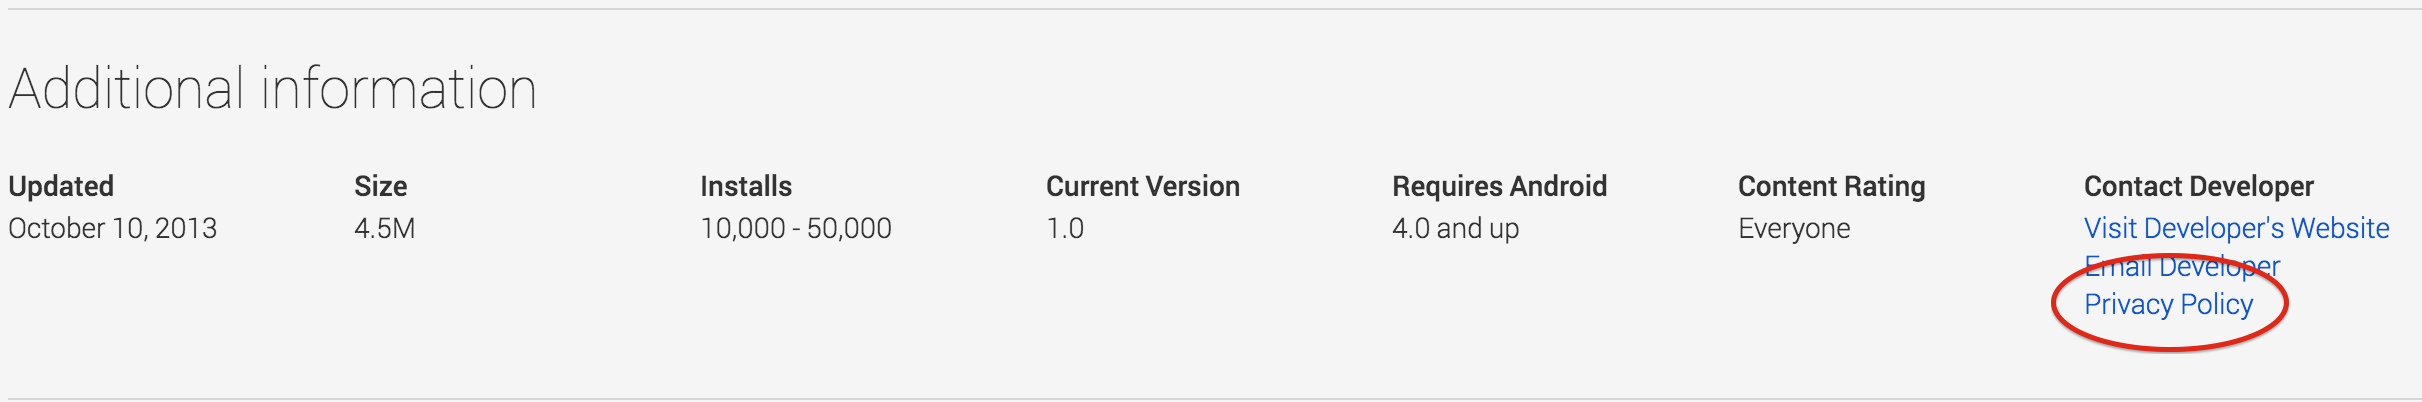
\includegraphics[width=\textwidth]{images/play-store-privacy-link}
      \caption{Privacy Policy link in the Play Store web interface}
      \label{fig:play-store-privacy-link}
\end{figure*}

However, while the \texttt{AndroidManifest.xml} file is guaranteed to be present for any application on the Play Store, this does not hold true for the Privacy Policy link. 

It is not in fact enforced by neither Play Store policies for an app to have a Privacy Policy at all. There is also no legal requirement (although deceptive practices are prohibited by the law).

So it two cases can occur: either the app does not have a Privacy Policy at all, or the developer has not inserted the Privacy Policy on the Play Store. In both cases the automatic retrieval of the Privacy Policy given an app is made impossible, so we will not further distinguish between them.

From the data we collected, it appears that out of the top 1093 downloaded free games apps, about the 39.79\% does not have a privacy policy publicly available through the Play Store.

% \todo[inline]{insert a pie chart here}

That being said, a Privacy Policy link is still no guarantee of the ability of retrieving a sensible Privacy Policy document. The link can point to anything the developer decides, and this leads to extremely heterogeneous paths to reach the final document of our interest.

The first issue encountered is the redirection mechanism that is very often in place. As an example, the Privacy Policy URL for \emph{Angry Birds}, by Zynga, is:

\url{https://www.google.com/url?q=http://m.zynga.com/about/privacy-center/privacy-policy}

which redirects to

\url{http://m.zynga.com/about/privacy-center/privacy-policy}

which redirects to

\url{http://company.zynga.com/privacy/policy}

which contains the Privacy Policy document.

% \todo[inline]{Talk about the Disney example}

%%%%%%%%%%%%%%%%%%%%%%%%%%%%%%%%%%%%%%%%%%
\subsection{Semantic analysis}
Once the document has been retrieved, it need to be semantically processed. For this purpose, we take advantage of Treat, a natural language processing framework for Ruby \cite{treat}. The Treat project aims to build a language-agnostic NLP framework for Ruby with support for tasks such as document retrieval, text chunking, segmentation and tokenization, natural language parsing, part-of-speech tagging, keyword extraction and named entity recognition.

The privacy policy document is firstly split into its logical subdivision using a SRX chunker, which implements the approach proposed in a study by Marcin Milkowski and Jaroslaw Lipski \cite{Milkowski:2009:USS:1987717.1987736}.

The the document is furthed split into sentences with the aid of a SRX segment, again proposed by Marcin Milkowski and Jaroslaw Lipski \cite{Milkowski:2009:USS:1987717.1987736}.


\begin{figure*}[t]
\centering
     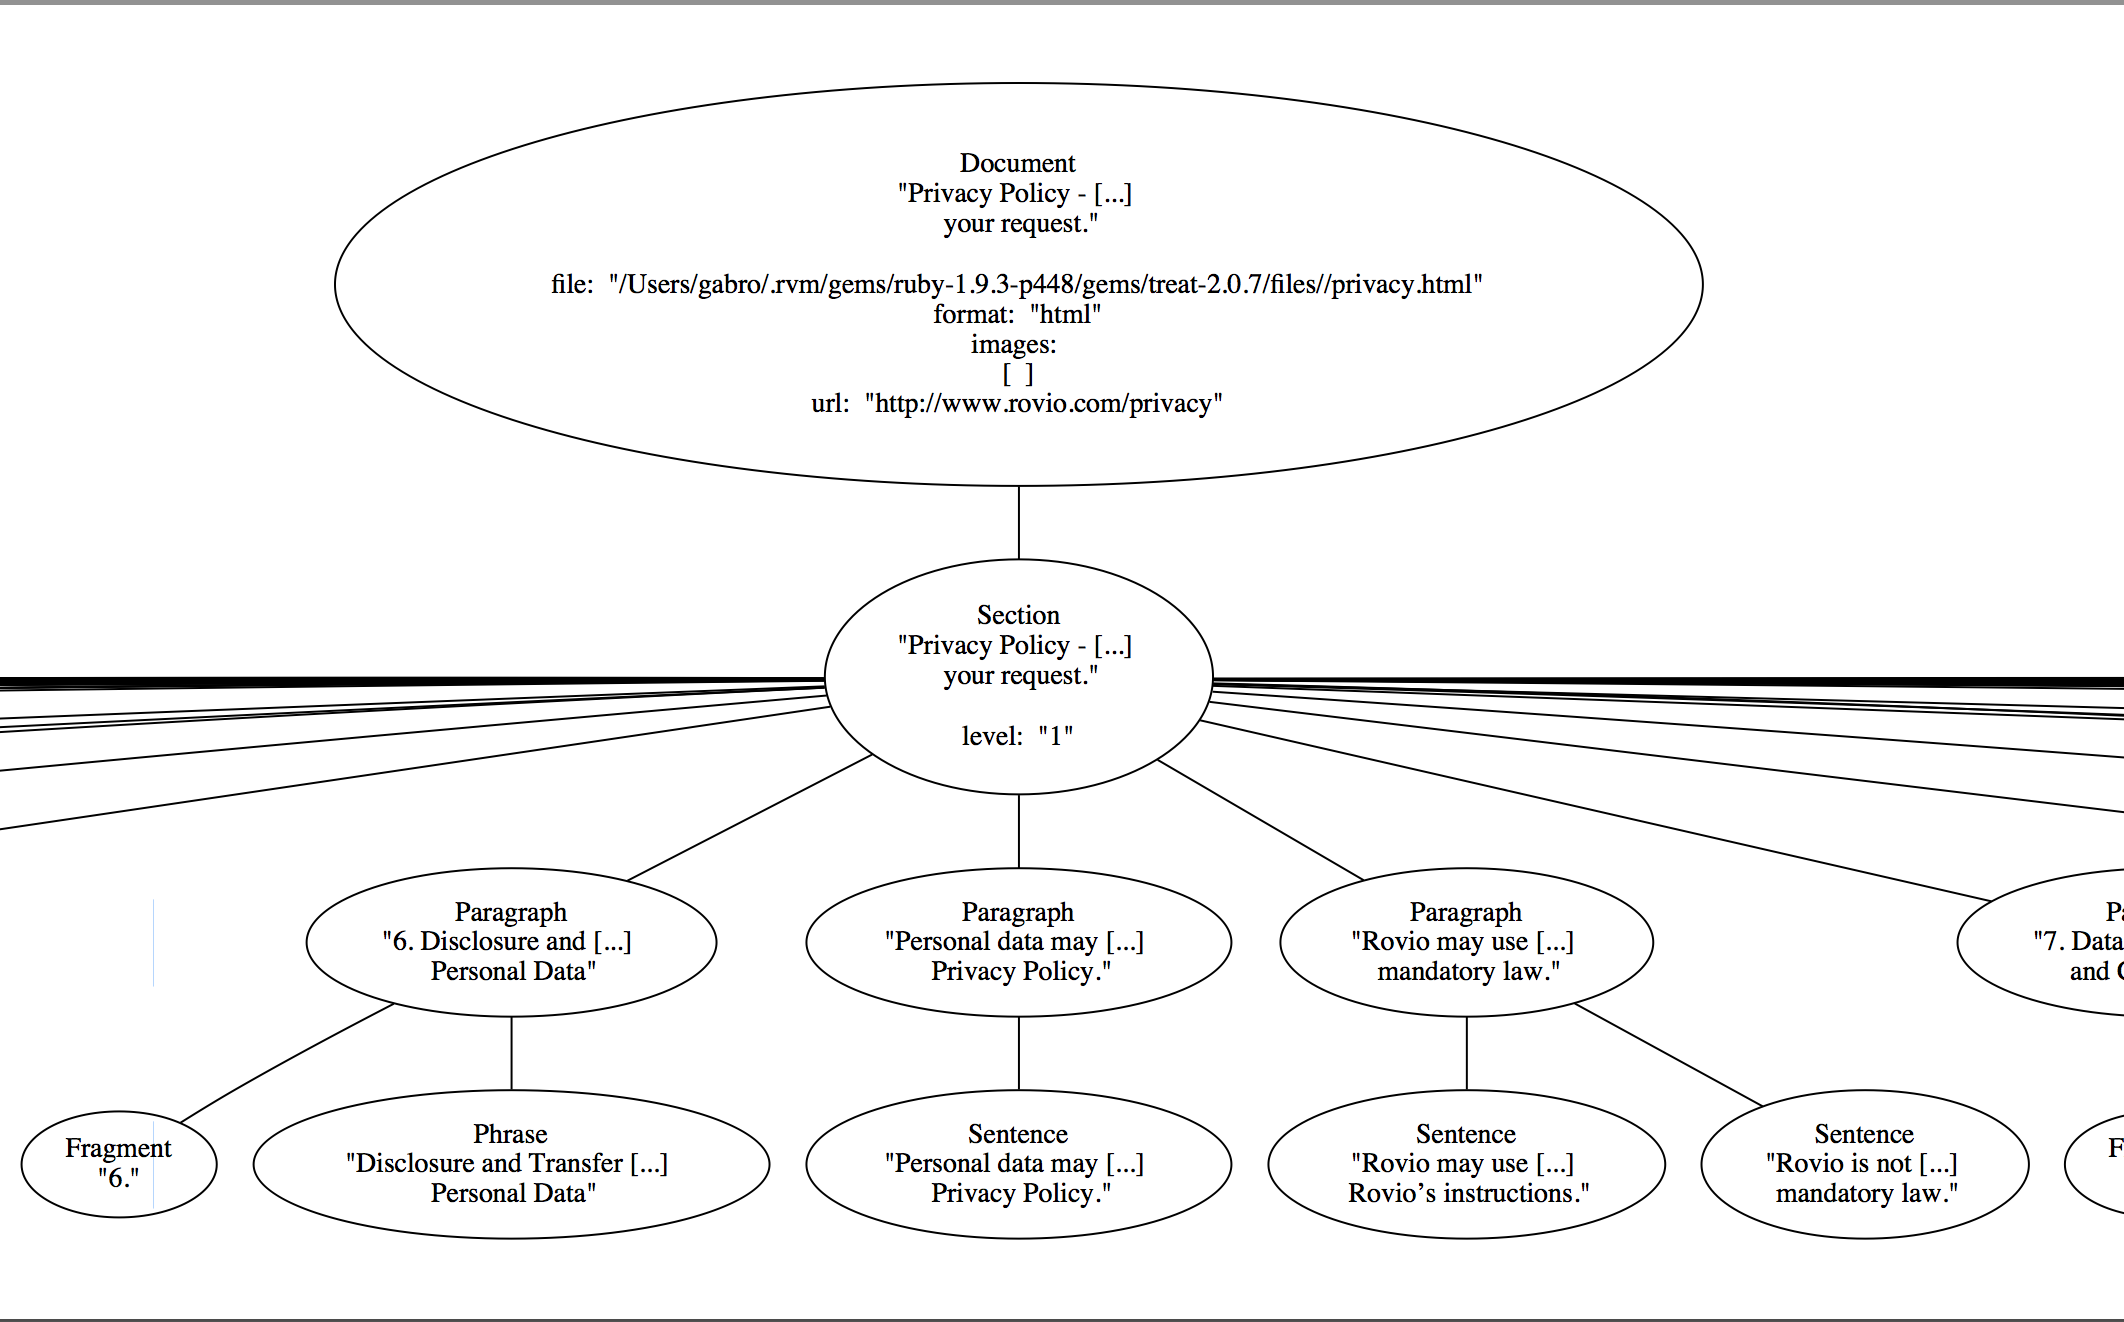
\includegraphics[width=\textwidth]{images/rovio-structure}
      \caption{Detail of Rovio's Privacy Policy structure}
      \label{fig:rovio-structure}
\end{figure*}

Figure \autoref{fig:rovio-structure} shows a detail of the semantic tree in which the original policy has been divided. Each internal node represents either paragraphs or sections of the document, whereas the leaf nodes are phrases and sentences.

Once sentences and phrases have been obtained, they can be searched for the expressions contained in the lookup table of each permission.
For example let us take the sentence.

\begin{quote}
{\emph{Rovio or third parties operating the ad serving technology may use demographic and \textbf{geo-location} information (for more information regarding use of Location Data see below Section 3) as well as information logged from your hardware or device to ensure that relevant advertising is presented within the Service.}}
\end{quote}

The lookup table of \texttt{ACCESS\_COARSE\_LOCATION} contains the word ``location'', hence the above sentence will be matched and will be considered relevant to such permission.

\subsection{Results collection}
Results are discussed in details in \autoref{sec:results}, however their collection brought up several technical challenges that required a rather sophisticated implementation to be dealt with. The main issue is represented by the significant number of applications we want to analyze; for each one of them we need to retrieve their privacy policy, their permission list and then analyze such information.

The challenges then become two:
\begin{itemize}
  \item Performing thousands of simoultaneous requests to Play Store servers
  \item Performing thousands of simoultaneous analysis on the same machine
\end{itemize}

The first challenge derives from Google's anti-bot protection, which result in a IP-ban in case of too many requests in a short amount of time.
The second challenges is instead an architectural limitation: spawning thousands of simultaneous computations easily hogs any personal computer's CPU, most likely leading to a system crash.

A naive approach to both challenges would be to serialize the operations, analyzing only one application at the time. Hoever, considering an average processing time of 10 seconds per application, analyzing thousands of applications would require several hours of computation and such architeture wouldn't scale within reasonable bounds in case of an increased number of applications (e.g. if one would like to analyze a significant fraction of the Play Store).

What we want is then a fixed amount of computations running concurrently, in order to achieve a fast computation without hogging computer's resources. We achieved this result taking a functional approach, namely utilizing Celluloid, a concurrent object oriented programming framework for Ruby.

Using Celluloid, we spawn a new computation for each thread - or in other terms, an \emph{actor} - which runs asynchronously and writes the results back on a MongoDB database. We use a fixed amout of actors, collectively referred to as a pool, in order to prevent the computation to use all the computer's resources and also to prevent to be banned from Google.
The result is a satisfying compromise between speed and available resources that allows to terminate the computation within reasonable time horizons.

\section{Quantitative results}
\label{sec:results}
In this section we present a metric used to evaluate the compliance of an application w.r.t. its privacy policy and we expose the quantitative results in terms of such metric.

\subsection{Metric definition}
\label{sec:metric}
We now define a metric to evaluate the goodness of one application with respect to its compliance to its privacy policy.

First, we manually assign to each privacy-related permission a score from 1 to 3, representing the severity of its potential impact on the user's privacy, where 1 signifies a permission with low impact and 3 signifies a permission carrying a very high danger.

Such scores are arbitrarily defined, in accordance with observation and existing literature on permission analysis,
and are shown in \autoref{tab:permission-scores}.

\begin{table}[ht]
    \caption{PERMISSION IMPACT SCORES}
    \label{tab:permission-scores}
    \centering
    \begin{tabular}{clc}
        \toprule
            \#   & Permission impact scores \\
            \midrule
                1  & INTERNET                       &   3 \\
                2  & READ\_EXTERNAL\_STORAGE        &   2 \\
                3  & WRITE\_EXTERNAL\_STORAGE       &   2 \\
                4  & ACCESS\_WIFI\_STATE            &   1 \\
                5  & READ\_PHONE\_STATE             &   3 \\
                6  & GET\_ACCOUNTS                  &   3 \\
                7  & ACCESS\_COARSE\_LOCATION       &   3 \\
                8  & GET\_TASKS                     &   1 \\
                9  & ACCESS\_FINE\_LOCATION         &   3 \\
                10 & READ\_LOGS                     &   1 \\
                11 & RECORD\_AUDIO                  &   2 \\
                12 & READ\_CONTACTS                 &   3 \\
        \bottomrule
    \end{tabular}
\end{table}

Secondly, we use the scores to compute a weighted sum of the number of permissions that lack an explicit mention in the privacy policy, formally defined in \autoref{eq:goodness-metric}

\begin{align}
\label{eq:goodness-metric}
  \sum\limits_{i=1}^n &= w_i p_i \\
  w_i &= \text{ score of the} i^{th} \text{permission} \\
  %
  p_i &=
  \begin{cases}
    & 0 \text{ if the permission is mentioned in the privacy policy} \\
    & 1 \text{ otherwise}
  \end{cases}
\end{align}

The final result is a metric estimating the compliance of an Android application to its own privacy policy. The lower the score, the more compliant the application.

We run the analysis on the same 4300 applications used to generate the top used permissions and the results are shown in \autoref{fig:results}

\begin{figure}[tb]
\centering
     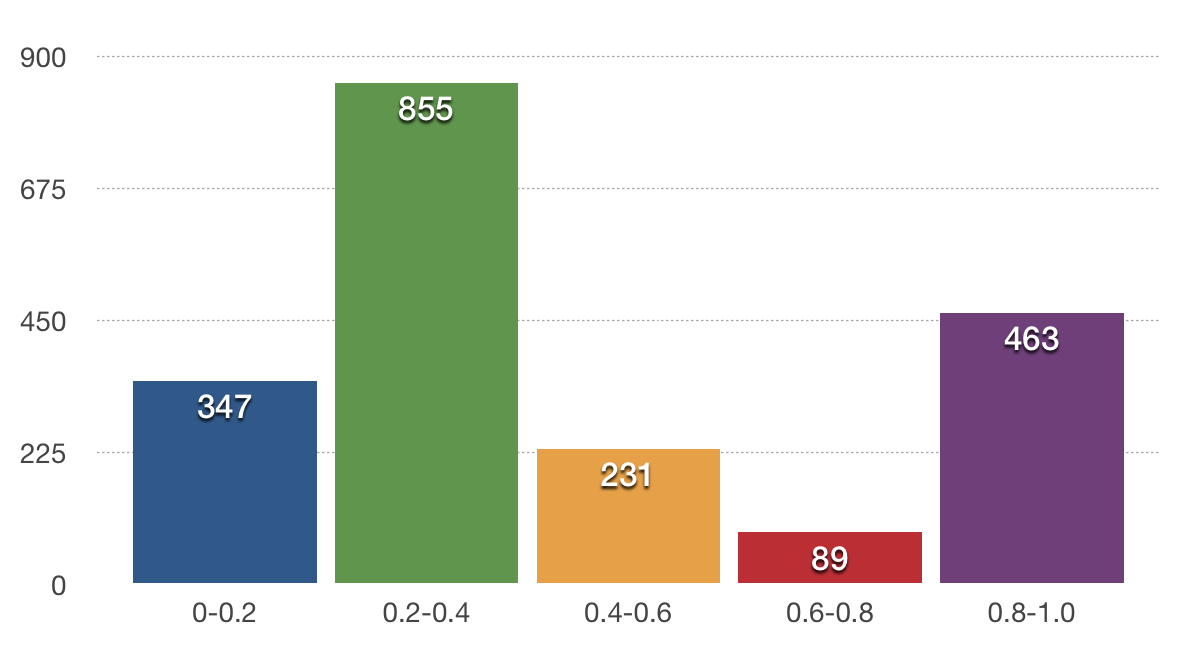
\includegraphics[width=\linewidth]{images/results}
      \caption{Quantitative results run over 4300 Android applications on December 7, 2013}
      \label{fig:results}
\end{figure}

\section{Qualitative results}
\label{sec:qualitative-results}
Out of the thousands of applications analyzed, we now focus our attention on a few notable cases.

\subsection{Case study: Shopkick}
Shopkick is a popular shopping rewards app and it is known \cite{shopkick-lifehacker} to require some sensitive permissions that should worry any user of this app. \autoref{tab:shopkick-permissions} show the complete list of permissions of the Android application.

\begin{table}[ht]
    \caption{SHOPKICK APP PERMISSIONS}
    \label{tab:shopkick-permissions}
    \centering
    \begin{tabular}{l}
        \toprule
            Permissions \\
            \midrule
                INTERNET \\
                ACCESS\_NETWORK\_STATE \\
                ACCESS\_COARSE\_LOCATION \\
                ACCESS\_FINE\_LOCATION \\
                READ\_PHONE\_STATE \\
                WRITE\_EXTERNAL\_STORAGE \\
                ACCESS\_WIFI\_STATE \\
                RECORD\_AUDIO \\
                CAMERA \\
                FLASHLIGHT \\
                VIBRATE \\
                BLUETOOTH \\
                GET\_ACCOUNTS \\
                RECEIVE\_BOOT\_COMPLETED \\
                READ\_CONTACTS \\
                CALL\_PHONE \\
                WAKE\_LOCK \\
                READ\_EXTERNAL\_STORAGE \\
                READ\_CALL\_LOG \\
        \bottomrule
    \end{tabular}
\end{table}

We can immediately spot a few permissions with a very high impact score, for example \texttt{RECORD\_AUDIO}, \texttt{CAMERA} and \texttt{ACCESS\_FINE\_LOCATION}.

\texttt{RECORD\_AUDIO} grants the application the ability to access the device's microphone to record audio, without any explicit consent by the user other than installing the app itself. This means that the app is virtually enabled to record audio at any time, with no possibility of being disabled. Especially in combination with the \texttt{RECEIVE\_BOOT\_COMPLETED} permission, that allows the app to be launched when the phone has booted, and the \texttt{INTERNET} permission, which enables sending data over the Internet, this is considerably worrying: an application could easily start itself as soon as the phone has been turned on, constantly record any sound going through the device's microphone and finally send everything over the Internet to a remote server, where the content can be stored and accessed in a later time.

To make things worse, the application also requests the permission \texttt{ACCESS\_FINE\_LOCATION}, meaning that the audio recording can be triggered according to the user's location, perhaps the workplace, home or other sensitive locations.

It is not hard to see how this capabilities can turn the app into a roving spyware, i.e. an application with whose hidden purpose is eavesdropping and spying on the device owners, let alone the people they are have contacts with.

Further investigations reveal how the app apparently uses the device's microphone in order to validate the physical location of the user in a store. According to the New York Times, \emph{The app knows someone is in a store by listening for an audio transmitter placed in each participating store; the phone’s microphone picks up the signal, which people cannot hear.}.

We can formalize a subset of this situation in terms of the representation previously discussed in \autoref{sec:intro}.
\begin{itemize}
    \item The permission \texttt{RECORD\_AUDIO} ($P_1$) enables the action \\ \emph{record\_audio\_from\_the\_device\_microphone} ($A\_1$);
    \item the permission \texttt{INTERNET} ($P\_2$) enables the action \\ \emph{send\_data\_over\_the\_internet} ($A\_2$);
    \item the permission \texttt{CAMERA} ($P\_3$) enables the action \\ \emph{record\_images\_from\_the\_device\_camera} ($A\_3$);
    \item the permission \texttt{ACCESS\_FINE\_LOCATION} enables the action \\ \emph{detect\_location\_of\_device} ($A_4$)
\end{itemize}

The combination of $A_1$ and $A_2$ enables the behavior \emph{validate\_presence\_in\_store} ($B\_1$). On the other hand $A\_1$, $A\_2$, $A\_3$ and $A\_4$ can also be combined enabling the behavior \emph{record\_audio\_and\_video\_when\_user\_is\_at\_home} ($B_2$).

Both behaviors result unexpected to the user, but while $B_1$ is probably considered legit - and even desirable -, $B_2$ is definitely unexpected, undesirable and possibly unlawful.

We now look at Shopkick's privacy policy looking for references of the aforementioned permissions.

\subsubsection{RECORD}
Our tool identifies this paragraph as relevant to the matter of recording audio:

\begin{quote}
{\emph{“(iv) record, determine or use information about or from another content delivery platform (for example, to unlock potential rewards or offers based on your watching of a specific a commercial or show that is broadcast on your television or on the web, the shopkick application may ask you to open the app while you are watching TV, and then \textbf{we may record or analyze the audio signal from the television set via the shopkick app and your cell phone’s microphone}, to determine the commercial, and/or program, including the date and/or time)}}
\end{quote}

A manual inspection of the policy confirms that this is indeed the relevant section and that the permissions is covered by the privacy policy.

\subsubsection{ACCESS\_FINE\_LOCATION}
Concerning the user's location, the tool identifies this sentence as relevant:

\begin{quote}
{\emph{(i) automatically record information that your mobile phone/device sends or transmits, including […] geographical location (if you consent to that)}}
\end{quote}

While it is true that the privacy policy covers this matter, it is also worth noting how the last phrase is misleading: as we saw before the user grants permissions at install time, on an Android device, so the consensus has already been given. Stating \emph{If you consent to do that} gives a sense of false assurance, when it is actually a tautology on the Android platform.

\subsubsection{CAMERA}
The tool signals that no references have been found in the privacy policy regarding the \texttt{CAMERA} permission and a manual inspections confirms that Shopkick's privacy policy doesn't mention in any way the use of the device's camera as a medium of acquiring data.

As it currently stands, Shopkick's application can collect any image from the user's camera without they being notified and the privacy policy does not restrict this by any mean.

Our tool successfully detected this behavior, helping in identifying a gap in the privacy policy of this popular application.

\section{Conclusions}
\label{sec:conclusions}
We presented a novel approach to the analysis of privacy policies in the context of Android applications. We introduced a framework for reasoning and proving properties of privacy policies, laying down the foundation for a new area of investigation.

The tool we implemented greatly eases the process of understanding the privacy implications of installing third party apps and it has already been proven able to highlight worrisome instances of applications.

The tool is developed with expandability in mind, and further developments in the approach can easily be integrated in order to increase the reliability and effectiveness.

\section{Future Work}
\label{sec:future-work}
This paper aims at laying the foundation for a new area of investigation, namely the relationship between mobile applications capabilities and behaviors and their privacy policies. As we mentioned in \autoref{sec:intro} several steps can be taken towards user awareness about privacy matters and this work covers the first necessary ones: identifying and analyzing the privacy-relevant permissions and examining their relationships with the privacy policies language. This enables further steps in the investigation and we now outline some of them.

\subsection{Live monitoring of behaviors}
As anticipated in the \autoref{sec:intro}, the first natural steps following the present work would be to live monitor the application's behavior. A static analysis can provide useful information about the \emph{potential} behaviors that can occur, but only a dynamic observation of applications running on real device can give insights about the \emph{actual} behaviors.

The first implementation one can think of is a passive monitoring of applications, with the final purpose of reporting such behaviors and further refine the ``goodness'' score presented in \autoref{sec:metric}.

One can also think of taking a step further and turn the monitoring into an active defense: if the application is found performing a behavior clearly in contrast with its privacy policy, the monitoring tool can immediately inform the user or even prevent such behavior from happening.

\subsection{Crowdsourced refinement of lookup tables}
One the main challenges of the current approach is reliably mapping privacy policies to permissions. The current implementation occasionally incurs in false positives and negatives. For example, if we consider the sentence:

\emph{Merchandise can only be shipped to approved U.S. shipping locations.}

taken from the aforementioned Shopkick's privacy policy, it is immediately evident to a human reader that, in this context, the word ``location'' does not refer to the collection of the user's location, whereas the current implementation considers it as such.

In order to face this challenges there are a few approaches one can think of doing: one of them is allowing the users of this tool to provide feedback on each sentence. They could either mark the sentence as \emph{relevant} or \emph{not relevant} and therefore improve the scoring of an application. The same approach could then be used to identify false negatives: relevant sentences can be not recognized and a user can signal such fact indicating which relevant portions of the privacy policy apply to the selected permission.

\subsection{Improved NLP}
As we mentioned above, a few approaches can be taken in order to refine the mapping of privacy policies to permissions. A complimentary approach to the aforementioned crowdsourced solution, is to improved the NLP analysis. For examples, the sentence structure can be taken into consideration. If we consider the previous example

\emph{Merchandise can only be shipped to approved U.S. shipping locations.}

one can think of a smarter classifier that identifies ``can be shipped'' as a verbal expression and recognizes it as semantically not relevant to privacy matters when used to refer to ``shipping locations''.

Such classifier would of course be much more complex to build, although simplified by the common patterns found in many privacy policies, that would make it more reliable.

%
% The following two commands are all you need in the
% initial runs of your .tex file to
% produce the bibliography for the citations in your paper.
\bibliographystyle{abbrv}
\bibliography{bibliography}  % sigproc.bib is the name of the Bibliography in this case
% You must have a proper ".bib" file
%  and remember to run:
% latex bibtex latex latex
% to resolve all references
%
% ACM needs 'a single self-contained file'!
%
\end{document}
